\documentclass[11pt,a4paper]{article}

\usepackage[T1]{fontenc}
\usepackage[utf8]{inputenc}
\usepackage{lmodern}
\usepackage[margin=1in]{geometry}
\usepackage{graphicx}
\graphicspath{{figures/}}
\usepackage{booktabs}
\usepackage{amsmath}
\usepackage{siunitx}
\usepackage{float}
\usepackage{xcolor}
\usepackage{caption}
\captionsetup{font=small,labelfont=bf}
\usepackage{enumitem}
\usepackage[hidelinks]{hyperref}
\usepackage{cleveref}
\usepackage{parskip}

\hypersetup{
  pdftitle={Exploratory Data Analysis of NHS England RTT Demand for Federated Forecasting},
  pdfauthor={Nilesh Sarkar},
}

\title{\textbf{Exploratory Data Analysis of NHS England\\ Referral-to-Treatment Demand}\\[0.4em]
\large A Data Foundation for Cross-Silo Federated Demand Forecasting}
\author{Nilesh Sarkar \\ \small fedOPD project}
\date{11 July 2026}

\begin{document}
\maketitle

% ===== section: front =====
\begin{abstract}
This report presents the exploratory data analysis (EDA) undertaken to verify, consolidate and characterise the data underpinning \emph{fedOPD}, a cross-silo federated forecasting system for NHS England Consultant-led Referral-to-Treatment (RTT) outpatient demand. Ninety-six monthly ``Full CSV'' releases spanning 2018-04--2026-03 (eight financial years, $160$--$196$k rows each) were audited for schema and integrity, then reduced through a fully ledgered canonical pipeline: keep RTT part type \texttt{Part\_3} (the exact new-periods demand signal), retain NHS trusts (three-character provider codes beginning \texttt{R\#\#}), drop the aggregate specialty \texttt{C\_999}, and sum over the commissioner split. The ledger traced $17{,}355{,}150$ raw rows down to $227{,}344$ canonical rows (\texttt{[date, branch, dept, demand]}) covering $194$ trusts, $24$ treatment functions and $3{,}243$ trust$\times$department monthly series, with $0$ duplicates removed and national totals externally validated in all four sentinel months (e.g.\ $1{,}544{,}011$ new periods in 2018-04). The characterisation returned four findings that directly shape the federated design: demand is heavily right-skewed (skew $4.92$; median $428$ vs.\ max $15{,}807$) with a robust per-trust scale spread of $66\times$ (p90/p10), making per-series scaling and size-aware client weighting mandatory; a strict balanced panel of $125$ of $194$ trusts reports in all $96$ months, giving a clean client set; the COVID shock is a shared regime, with national demand collapsing to $\sim$$31\%$ of baseline in 2020-04 before recovering to $\sim$$116\%$ by 2026-03; and trusts co-move strongly (median pairwise correlation $0.63$ on the largest department) while $38\%$ of long series carry a clear annual cycle. This combination of common national structure and heterogeneous per-trust scale and casemix is precisely the regime in which \emph{personalised} federated learning (FedAvg/FedProx with client personalisation) is expected to outperform both a single global model and isolated per-trust models, confirming that the data supports the intended cross-silo forecaster.
\end{abstract}

\tableofcontents
\clearpage


\section{Introduction}\label{sec:intro}

\subsection{The operational problem}
NHS England publishes Consultant-led Referral-to-Treatment (RTT) waiting-time statistics monthly, recording, for each provider and each treatment function, the volume of care pathways at each stage of the waiting process. The count of \emph{new} RTT periods (RTT part type \texttt{Part\_3}, column \texttt{Total All}) is an operational measure of incoming outpatient demand: how many new referral pathways a department must absorb in a given month. Planning capacity against this demand---clinic slots, workforce, and service-line allocation---is an operations-research problem, not a clinical one, and the object to be learned is a per-department \emph{demand forecaster} rather than any patient-level model. Accurate month-ahead forecasts, disaggregated to the trust$\times$treatment-function grain, would let providers and their commissioners plan under uncertainty instead of reacting to realised backlogs. The eight-year window studied here is deliberately chosen to span the 2020 COVID collapse and the subsequent recovery, so that any forecaster is characterised against the largest demand shock in the record rather than a placid baseline.

\subsection{Why federated learning fits}
Every NHS trust reports its RTT activity upward through the same national return, which makes the many providers natural collaborators on a shared forecasting task. Yet the underlying operational data cannot simply be pooled into one central training set: it originates at, and is governed by, individual trusts, and the design principle of \emph{fedOPD} is that a trust's raw records never leave the site. Federated learning resolves this tension directly. Each trust acts as a cross-silo \emph{client} that trains a local copy of a shared per-department forecaster on its own data; only model updates---never raw referral counts---are exchanged with a coordinator that aggregates them into a global model. Because the providers report the same signal in the same schema (verified here as stable across the eight-year window despite the file growing from $69$ to $121$ columns), the clients are learning a common object, while the strong cross-trust co-movement documented in this EDA (median pairwise correlation $0.63$) confirms there is genuine shared structure for a federated model to exploit.

\subsection{Two coupled planes over one hierarchy}
The system is organised as two coupled planes running over the same provider hierarchy (NHS England $\rightarrow$ region $\rightarrow$ ICB $\rightarrow$ trust $\rightarrow$ department). The \emph{federated-learning plane} learns the forecast: the global model flows down to the trusts and model updates flow back up, optionally aggregated hierarchically (trust $\rightarrow$ ICB/region $\rightarrow$ HQ). The \emph{agentic plane} acts on the resulting forecasts, turning predicted demand into capacity, staffing and service-line decisions, with allocations flowing down and resource requests flowing up. The two planes branch on provider type only in the acting plane: capacity is \emph{allocated} to NHS trusts, whereas independent providers can only be \emph{commissioned} (bought from). This report concerns the foundation both planes stand on---the data---and in particular scopes the forecasting plane to NHS trusts, whose $\texttt{R\#\#}$ codes were isolated during the canonical build.

\subsection{Objectives and contributions of this EDA}
This EDA has three objectives, each a prerequisite for the modelling work that follows. First, to \emph{verify} the raw data end to end: confirming the schema, part-type vocabulary and integrity of all $96$ monthly files, and externally validating the extracted national demand totals against published figures. Second, to \emph{build the canonical table} through a single, transparent and fully ledgered pipeline that reduces $17{,}355{,}150$ raw rows to $227{,}344$ canonical rows keyed on \texttt{[date, branch, dept, demand]}, saved as a reproducible artefact. Third, to \emph{characterise} the resulting panel well enough to drive the two downstream design decisions: which trusts and departments constitute a sound federation client set (the balanced-panel and coverage analysis), and how the forecaster must be shaped to cope with the data's heavy skew, wide per-trust scale spread, structural sparsity, COVID regime shift and annual seasonality. The remainder of the report follows the eight EDA stages that deliver these objectives, and closes with the evidence that the data supports a personalised federated forecaster.

% ===== section: data =====
\section{Data and Provenance}\label{sec:data}

The study draws on a single public source: the NHS England Consultant-led
Referral-to-Treatment (RTT) waiting-times statistics, published monthly as the
``Full CSV'' extract. Each file is a complete, un-aggregated snapshot of RTT
activity for one calendar month, reported by provider, by commissioner, by
treatment function, and by RTT part type. The collection used here spans
96 consecutive monthly files covering the eight financial years
2018-04--2026-03. The files are large and non-stationary in shape: each
carries roughly 160,000--196,000 rows, the column count steps from 69 to 121,
the number of reporting providers grows from 417 to 533, and the number of
treatment functions grows from 20 to 24 over the window. All of this
operational structure is present without any patient-level information --- the
data record departmental \emph{demand}, never clinical records, which is what
makes the source appropriate for an operations-research forecasting task.

\subsection{Window: why 96 files, and why the 2018-04 floor}

Two boundary decisions define the window. The \emph{floor} at 2018-04 is a hard
compatibility constraint: files earlier than April 2018 use an incompatible
older ``SHA \& Self Trusts'' layout whose columns and organisational coding do
not align with the modern extract, so 2018-04 is the earliest month that can be
loaded under one stable schema. The \emph{length} of eight years is a
deliberate modelling choice rather than mere availability: it brackets the
COVID-19 shock end to end. The national Part\_3 total collapses from a
2018-04 baseline of 1,544,011 to a trough of 474,295 in 2020-04 --- about
31\% of baseline --- before recovering to 1,783,457 by 2026-03 (roughly
116\% of baseline). Capturing the collapse, the recovery, and the subsequent
above-baseline growth in full is essential, because a forecaster trained only
on the post-recovery regime would never see the largest demand movements in the
record and would be blind to the shared national shock that the federated model
is meant to exploit.

\subsection{Canonical target table}

The raw extract is reduced to a single canonical table at the grain of one row
per trust $\times$ treatment function $\times$ month, with schema
\texttt{[date, branch, branch\_name, icb, dept, dept\_name, demand]}. The
learnable target is \texttt{demand}: the RTT \texttt{Part\_3} (``New RTT
Periods'') \texttt{Total All} count, summed over the commissioner split. Four
filter rules produce this table: keep only rows with \texttt{RTT Part Type ==
Part\_3}; keep only NHS trusts, identified by a 3-character
\texttt{Provider Org Code} beginning with \texttt{R} (independent providers use
5-character codes and are excluded); drop the aggregate ``Total'' treatment
function \texttt{C\_999}; and sum over the commissioner dimension so that each
trust $\times$ department $\times$ month appears exactly once. The \texttt{date}
key is parsed case-insensitively from the \texttt{Period} field, because the
month token is title-cased in some eras and upper-cased in others (see
\Cref{tab:dict}). Only 9 source columns are needed to build the entire
canonical table; the remaining columns (chiefly the weekly wait-band histogram)
are not read.

\begin{table}[H]
\centering
\caption{Canonical data dictionary: the 9 source columns of the RTT Full CSV,
their canonical role, and the canonical output field each maps to.}
\label{tab:dict}
\small
\begin{tabular}{lll}
\toprule
Source column (RTT Full CSV) & Canonical role & Output field \\
\midrule
Period                   & key      & \texttt{date} \\
Provider Org Code        & key / filter & \texttt{branch} \\
Provider Org Name        & hierarchy & \texttt{branch\_name} \\
Provider Parent Org Code & hierarchy & \texttt{icb} \\
Provider Parent Name     & hierarchy & (ICB label) \\
Treatment Function Code  & key / filter & \texttt{dept} \\
Treatment Function Name  & hierarchy & \texttt{dept\_name} \\
RTT Part Type            & filter   & (selects \texttt{Part\_3}) \\
Total All                & measure  & \texttt{demand} \\
\bottomrule
\end{tabular}
\end{table}

The role assignment in \Cref{tab:dict} is what makes the pipeline auditable.
\texttt{Period}, \texttt{Provider Org Code}, and \texttt{Treatment Function
Code} form the composite key \texttt{[date, branch, dept]}; \texttt{RTT Part
Type} is a pure selection filter that contributes no output field;
\texttt{Total All} is the sole measure and becomes \texttt{demand}. The
hierarchy fields carry the federation's organisational structure --- the
provider name, its parent (used as the ICB identifier and its label), and the
treatment-function name. The department is keyed on the \emph{code}
(\texttt{dept}) rather than the name, because treatment-function \emph{names}
drift across eras while the codes are stable; the name is retained only as a
human-readable annotation.

\subsection{Sentinel months}

Rather than exhaustively re-inspecting all 96 files at every schema check, four
\emph{sentinel} months were used for development and integrity testing, chosen
to bracket every known source of structural variation. Two are the window
\emph{endpoints}: 2018-04, the oldest month in the modern layout
(69 columns, 196,340 rows), and 2026-03, the newest (121 columns,
183,400 rows). One marks the known schema \emph{break}: 2021-04, the month at
which the column layout steps from 69 to 121 (160,251 rows), extending the
weekly wait-band histogram from 52 to 104 weeks to accommodate the post-COVID
backlog. The last marks the known demand \emph{shock}: 2020-04, the COVID
collapse (69 columns, 125,460 rows), the month whose Part\_3 national total
falls to about 31\% of the 2018-04 baseline. Together these four months exercise
both extremes of column count, both era conventions for the \texttt{Period}
month case, and the full demand range from trough to peak, giving a small but
representative set on which the loader and its filters were validated before
being run across all 96 files.

% ===== section: method =====
\section{Methodology}\label{sec:method}

This section describes how the raw NHS England Referral-to-Treatment (RTT) statistics were audited, reduced to a single canonical table, and validated. The design goal throughout was accountability: every reduction step was ledgered, every national total was checked against an independently computed reference, and the entire analysis was made reproducible from a single notebook. Because the objective is cross-silo federated forecasting in which each NHS trust is a client whose raw data never leaves the site, the exploratory phase had to establish not only that the data are clean but also that they are \emph{structurally consistent across sites and time} --- a precondition for any shared model to be learnable.

\subsection{Sentinel-first workflow}
The corpus comprises 96 monthly ``Full CSV'' files spanning 2018-04--2026-03 (eight financial years), each carrying roughly 160,000--196,000 rows and, over the window, growing from 69 to 121 columns. Loading all 96 files repeatedly during development would have been both slow and wasteful, so the analysis adopted a \emph{sentinel-first} strategy: four months were chosen to bracket every axis of variation and all iterative development was carried out on those four alone. The sentinels were 2018-04 (the oldest file and the first month in the modern layout, 69 columns, 196,340 rows), 2020-04 (the COVID demand collapse, 69 columns, 125,460 rows), 2021-04 (the layout step to 121 columns, 160,251 rows), and 2026-03 (the newest file, 121 columns, 183,400 rows). Together these span both column layouts, the pre-COVID baseline, the pandemic trough, and the recovered present, so a rule that behaves correctly on all four is very likely to behave correctly on the remaining 92 months.

Full 96-file passes were reserved for the two tasks that intrinsically require every file: a \emph{schema audit} (confirming that the seven canonical fields, the single parent-header variant \texttt{Provider Parent Org Code}, and a numeric \texttt{Total All} are present in all 96 files) and a \emph{content sweep} (the actual canonical build). This separation kept iteration cheap while ensuring that no month escaped verification.

\subsection{Canonical construction pipeline}
The forecasting target is monthly new-referral demand per trust per treatment function. From each raw file the pipeline read only the nine columns needed to derive the canonical schema (\texttt{Period}; \texttt{Provider Org Code}; \texttt{Provider Org Name}; \texttt{Provider Parent Org Code}; \texttt{Provider Parent Name}; \texttt{Treatment Function Code}; \texttt{Treatment Function Name}; \texttt{RTT Part Type}; \texttt{Total All}) and applied a fixed sequence of filter rules to produce the canonical table \texttt{[date, branch, branch\_name, icb, dept, dept\_name, demand]}, one row per trust $\times$ treatment-function $\times$ month:

\begin{enumerate}[nosep]
  \item \textbf{Demand signal:} keep only rows with \texttt{RTT Part Type == Part\_3} (New RTT Periods), the exact demand label. This part type is present and identically named in every era, so the signal definition is stable across the full window.
  \item \textbf{Provider filter:} keep only NHS trusts, identified by a three-character \texttt{Provider Org Code} beginning with ``R''. Provider-code lengths are strictly $\{3,5\}$, independent providers carrying the five-character form, so the length-plus-prefix test is unambiguous.
  \item \textbf{Drop the aggregate specialty:} remove \texttt{Treatment Function Code == C\_999}, the ``Total'' pseudo-specialty, to avoid double-counting demand already represented by the individual treatment functions.
  \item \textbf{Sum over commissioners:} group by \texttt{[date, branch, dept]} and sum \texttt{Total All} across the commissioner split, since demand is defined at the provider--department level, not per commissioner.
  \item \textbf{Date parse:} map \texttt{Period} to a month-start date, parsing \emph{case-insensitively} because the month token is non-monotonic across the window (observed as April / APRIL / APRIL / March across the four sentinels); the title-cased month matched the filename in all four cases.
  \item \textbf{Type coercion:} convert \texttt{Total All} with a numeric coercion (\texttt{to\_numeric}, coerce) to guard against any stray non-numeric token, although the field was already \texttt{int64} with zero missing values in every era.
\end{enumerate}

Applying this pipeline across all 96 files reduced 17,355,150 raw rows to the final table in four ledgered stages (\Cref{sec:results}): the \texttt{Part\_3} filter retained 3,614,127 rows (20.8\% of raw), the trust filter retained 2,987,812 (82.7\% of \texttt{Part\_3}), dropping \texttt{C\_999} left 2,376,866, and the commissioner sum collapsed these to \textbf{227,344} canonical rows. Zero duplicate rows were removed. The finished table covers 96 months, 194 distinct trusts (the union across the window), 24 treatment functions, and 56 raw parent (ICB) codes, and was persisted as a single Parquet artifact.

\subsection{Accountability devices}
Four devices were built into the pipeline so that every claim in this report is auditable.

\paragraph{Filter ledger.} Each stage of the reduction recorded its input and output row counts (the figures above), so the path from 17,355,150 raw rows to 227,344 canonical rows is fully traceable and any future change to a filter rule can be diffed against a known baseline.

\paragraph{External validation.} Four national \texttt{Part\_3} totals --- computed independently from the raw files under the same filter definition (trusts only, drop \texttt{C\_999}, sum commissioners) --- were used as a reference: 2018-04 $=$ 1,544,011; 2020-04 $=$ 474,295; 2021-04 $=$ 1,394,578; 2026-03 $=$ 1,783,457. The pipeline's computed totals matched these references in all four cases (4/4), both from the raw sentinels and re-derived from the finished canonical table, confirming that no demand was gained or lost during reduction. The trough total 474,295 is $\approx 31\%$ of the 2018-04 baseline, quantifying the COVID collapse the eight-year window was specifically extended to capture.

\paragraph{Robust outlier detection.} Anomalies were identified with a robust rolling-median plus median-absolute-deviation (MAD) z-score, flagging observations with $|z| > 4$ on any series with at least 36 months of history. This robust estimator was preferred over a mean/standard-deviation rule precisely because the series contain large genuine shocks (the COVID regime) that would inflate a non-robust scale estimate and mask ordinary reporting anomalies. The detector raised 4,183 flags, concentrated in the expected months (354 in 2020-04, 218 in 2020-05, 209 in 2023-12 coinciding with the December 2023 industrial action).

\paragraph{Outlier register.} Every flag was written to a persistent register with a first-pass class (spike, drop, or COVID) so that downstream modelling decisions --- COVID months become a regime-flag feature and are kept; reporting spikes and drops are flagged and excluded from scaler fitting but kept; genuine surges are kept untouched; nothing is deleted --- rest on an explicit, inspectable audit trail rather than ad-hoc filtering.

\subsection{Reproducibility and environment}
The entire analysis lives in a single notebook that runs restart-and-run-all cleanly (57 cells, 0 errors), so the numbers in this report can be regenerated end to end without manual intervention. The canonical table was materialised once to a compact columnar artifact (\texttt{reports/tables/rtt\_canonical.parquet}, 0.6\,MB) that all later stages consume, decoupling the expensive 96-file build from the cheaper analytical passes and guaranteeing that every stage sees identical inputs. The work ran on a Linux server with an NVIDIA A100 80\,GB GPU exposed through a MIG \texttt{7g.80gb} instance, under Python 3.10 with pandas 2.3.3 and NumPy 2.2.6. Version pinning, the single-notebook constraint, the filter ledger, the 4/4 external validation, and the outlier register together make the reduction from raw NHS files to canonical demand table fully reproducible and independently checkable --- the standard of evidence required before trusting these series as the training data for a federated model whose behaviour cannot later be inspected site by site.

% ===== section: schema =====
\section{Results}\label{sec:results}
The following subsections report the findings of EDA stages~2--7, each quantified and cross-referenced to the figures and tables it produced.

\subsection{Schema Integrity and Verification}\label{sec:schema}

Before any demand series could be trusted, the eight-year monthly corpus was audited for schema stability and for the correctness of the demand-extraction filter. Four sentinel months were used for deep inspection --- 2018-04 (the oldest month in the modern layout), 2020-04 (the COVID collapse), 2021-04 (a schema step) and 2026-03 (the newest month) --- and every structural finding was then re-checked across all 96 files. \Cref{tab:sentinels} summarises the sentinel structure and \Cref{tab:validation} records the external validation of the demand filter.

\textbf{Column layout (F-01).} The per-file column count is not constant: it steps from 69 to 121 columns exactly at 2021-04. The boundary is clean, with 36 months at 69 columns (2018-04--2021-03) and 60 months at 121 columns (2021-04--2026-03). The 52 additional columns extend the weekly wait-band histogram from 52 to 104 weeks, i.e. the schema itself widened to record post-COVID waits beyond one year. This matters for the loader because it must not assume a fixed column set; the nine canonical fields, however, are present in both eras, so demand extraction is invariant to the step.

\textbf{RTT part types (F-02).} The set of part types $\{$\texttt{Part\_1A}, \texttt{Part\_1B}, \texttt{Part\_2}, \texttt{Part\_2A}, \texttt{Part\_3}$\}$ is identical across all eras, with \texttt{Part\_2A} already present from 2018-04 and nothing added later. \texttt{Part\_3} (New RTT Periods) is therefore an unambiguous, era-stable demand label, which is essential given that the forecasting target must mean the same thing in every training month.

\textbf{Treatment functions and the aggregate (F-03).} The number of treatment functions grows from 20 (2018-04, 2020-04) to 24 (2021-04, 2026-03). The aggregate ``Total'' specialty \texttt{C\_999} appears in every era and is dropped by the filter so that per-department demand is never double-counted against the specialty total.

\textbf{Provider structure (F-04).} Provider organisation codes take exactly the lengths $\{3,5\}$, cleanly separating NHS trusts (\texttt{R\#\#}, three characters) from independents (five characters). Across the sentinels the trust count \emph{shrinks} (184, 173, 170, 149) while the total provider count \emph{grows} (417, 414, 431, 533). The shrinking trust count reflects NHS trust mergers and consolidation over the window, whereas the growing provider total is driven by independent-sector expansion; the divergence confirms that the client population (trusts) must be tracked as a union across time rather than assumed fixed.

\textbf{Period case (F-05).} The textual month case in the \texttt{Period} field is non-monotonic across the sentinels (\emph{April}, \emph{APRIL}, \emph{APRIL}, \emph{March}), so a case-sensitive date parse would fail on part of the corpus. A case-insensitive parse recovers the month in every file, and the title-cased month matched the source filename in 4 of 4 sentinels, providing an independent cross-check on the date key.

\textbf{Demand dtype (F-06).} The \texttt{Total All} field is stored as \texttt{int64} in every era with 0 \texttt{NaN} values, so demand is an exact integer count with no missing entries at source; any later \texttt{NaN} arises only when a series is reindexed to a full monthly frequency, not from the raw files.

\begin{table}[H]
\centering
\caption{Sentinel-month schema and provider structure.}
\label{tab:sentinels}
\small
\begin{tabular}{l r r r r r}
\toprule
Month & Rows & Cols & Treatment functions & NHS trusts (\texttt{R\#\#}) & Total providers \\
\midrule
2018-04 & 196,340 & 69  & 20 & 184 & 417 \\
2020-04 & 125,460 & 69  & 20 & 173 & 414 \\
2021-04 & 160,251 & 121 & 24 & 170 & 431 \\
2026-03 & 183,400 & 121 & 24 & 149 & 533 \\
\bottomrule
\end{tabular}
\end{table}

\textbf{External validation of the demand filter (F-07).} Applying the demand rule (keep \texttt{Part\_3}; keep NHS trusts; drop \texttt{C\_999}; sum over the commissioner split) and comparing the resulting national total against the independently verified NHS England figure yielded an exact match in 4 of 4 sentinels (\Cref{tab:validation}). The COVID trough at 2020-04 of 474,295 is $\approx 31\%$ of the 2018-04 baseline of 1,544,011, quantifying the scale of the pandemic collapse in new referrals and confirming that the filter reproduces official totals rather than an internally consistent but incorrect artefact.

\begin{table}[H]
\centering
\caption{External validation of the demand filter (national \texttt{Part\_3} totals).}
\label{tab:validation}
\begin{tabular}{l r r l}
\toprule
Month & Computed \texttt{Part\_3} total & Verified total & Status \\
\midrule
2018-04 & 1,544,011 & 1,544,011 & OK \\
2020-04 & 474,295   & 474,295   & OK \\
2021-04 & 1,394,578 & 1,394,578 & OK \\
2026-03 & 1,783,457 & 1,783,457 & OK \\
\bottomrule
\end{tabular}
\end{table}

\textbf{Full-window generalisation (F-08).} The sentinel findings were confirmed to hold across every file: the seven canonical fields required for the loader are present in 96 of 96 months, the parent-organisation header appears as a single variant (``Provider Parent Org Code'') with no competing spellings, and both \texttt{Part\_3} rows and a numeric \texttt{Total All} column are present in 96 of 96 files, giving 0 problem files. The schema is therefore verified as stable enough --- and the demand filter as externally correct --- for the canonical table to be built with confidence, which is a precondition for treating each trust as a comparable federated client.

% ===== section: canonmiss =====
\subsection{Canonical Construction}\label{sec:canon}

The canonical table was built by applying the locked filter rules of the study to all 96 monthly Full-CSV files in one pass. Each stage was ledgered so that the reduction from 17.4 million raw rows to the analysis table is fully auditable. \Cref{tab:ledger} records the row count surviving each step.

\begin{table}[H]
\centering
\caption{Filter ledger (96 months)}\label{tab:ledger}
\begin{tabular}{lrl}
\toprule
Step & Rows & Note \\
\midrule
Raw & 17,355,150 & all rows across 96 files \\
\texttt{Part\_3} & 3,614,127 & 20.8\% of raw (demand label) \\
NHS trusts & 2,987,812 & 82.7\% of \texttt{Part\_3} (\texttt{R\#\#} codes) \\
Drop \texttt{C\_999} & 2,376,866 & remove aggregate ``Total'' specialty \\
Canonical & 227,344 & sum over commissioners \\
\bottomrule
\end{tabular}
\end{table}

Two reductions dominate the ledger. First, restricting the RTT part type to \texttt{Part\_3} discards 79.2\% of rows, because a single file carries five part types and only \texttt{Part\_3} (New RTT Periods) is the demand signal of interest; keeping NHS trusts then removes the independent-sector providers, retaining 82.7\% of the \texttt{Part\_3} rows. Second, and more importantly, the collapse from 2,376,866 rows (after dropping \texttt{C\_999}) to 227,344 canonical rows -- a further $10.5\times$ compression -- is \emph{not} a filter at all but the group-and-sum over the commissioner split: the raw files record demand at the trust $\times$ department $\times$ \emph{commissioner} $\times$ month grain, whereas the forecasting target is defined at the trust $\times$ department $\times$ month grain. Summing over commissioners removes a purely administrative dimension that is irrelevant to a provider-side demand forecaster, and it is the correct grain for a client-per-trust federation. The deduplication check removed 0 rows, confirming the grouping keys are unique.

The finished canonical table holds 227,344 rows spanning 96 months (2018-04--2026-03), 194 trusts (union across the window), 24 departments, and 56 ICBs (the raw union of parent codes, later reconciled to 42 on the latest-month mapping). National monthly totals recomputed from the finished table matched the externally validated figures on all four sentinel months (4/4), and the table was persisted as a 0.6\,MB parquet file (\texttt{reports/tables/rtt\_canonical.parquet}) that serves as the single input to every downstream stage.

\subsection{Missing Data}\label{sec:missing}

Because the canonical grain is trust $\times$ department $\times$ month, ``missingness'' in this dataset is dominated by \emph{absent rows} -- trusts or departments that simply did not report in a given month -- rather than by corrupt or null values. This distinction is central to the federated design: a client that is present for only part of the window cannot be treated identically to one with a complete history.

\begin{figure}[H]
\centering
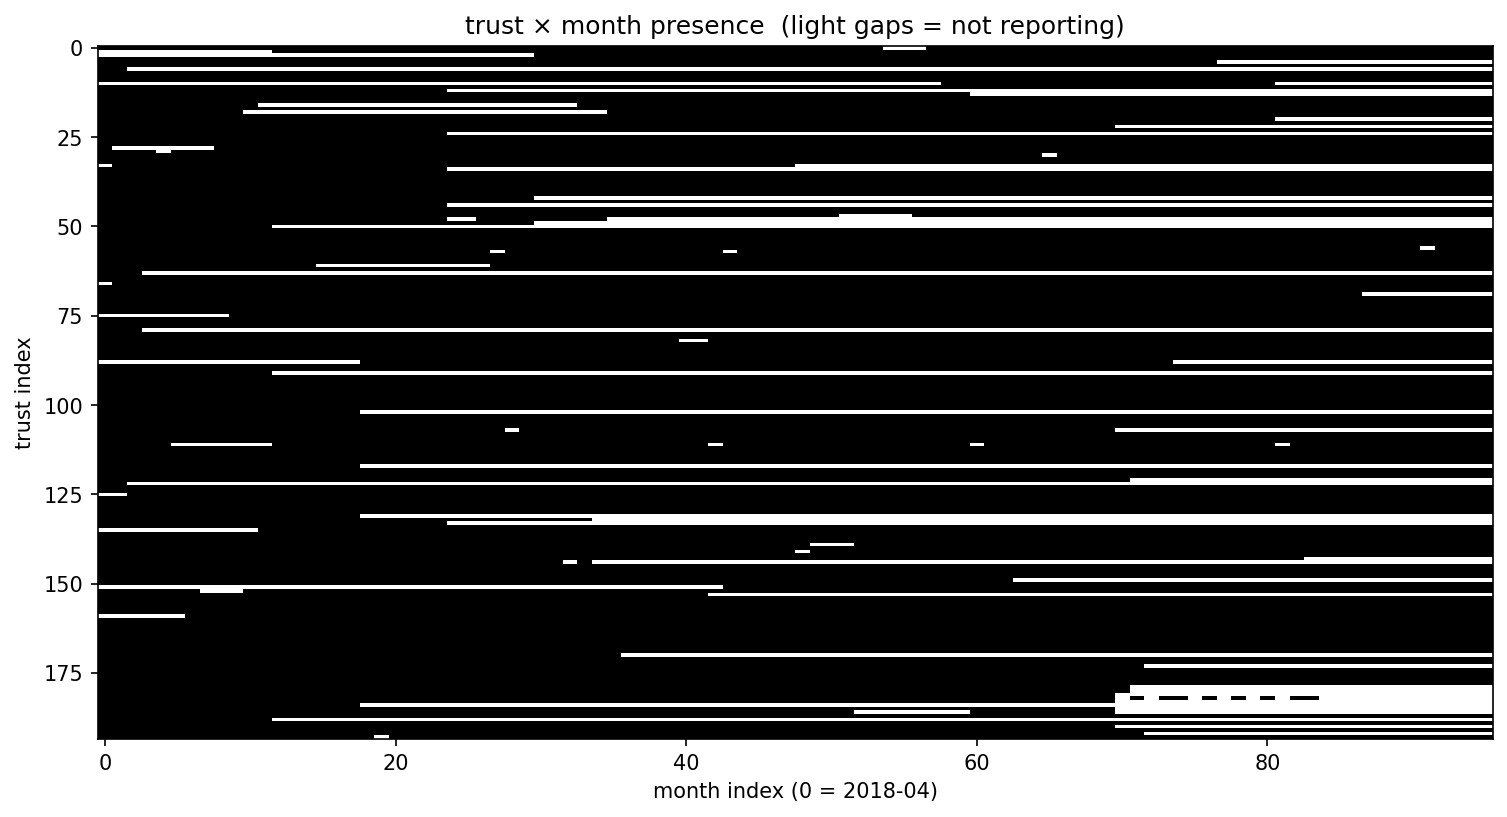
\includegraphics[width=0.85\linewidth]{figures/03_presence_heatmap.png}
\caption{Trust $\times$ month reporting presence; dark = reported.}\label{fig:presence}
\end{figure}

At the trust level (F-11), only 125 of the 194 trusts reported in all 96 months, forming a fully balanced panel; the remaining 69 have partial histories. Decomposing the incomplete trusts (F-12), 11 entered late while 45 exited early, so exits outnumber entries roughly four to one. The pattern in \Cref{fig:presence} is therefore not random attrition but structural: early-exit trusts reflect NHS trust mergers and consolidation, in which a provider code is retired and its activity is absorbed by a successor. This shapes client selection directly -- a stable federation panel must be drawn from the trusts that persist across the window.

At the finer trust $\times$ department grain (F-13), the 194 trusts and 24 departments yield 3,243 realised series. Of these, 1,412 (44\%) are complete across all 96 months, while 1,831 are gappy with a median coverage of 60 of 96 months. The number of departments a trust offers (F-14) ranges from a minimum of 1 to a median of 20 and a maximum of 24 (the full set), so casemix breadth varies widely across providers; the roughly 1,400 trust $\times$ department pairs that never appear are structural zeros (services a trust does not provide), not missing observations. Crucially, within the canonical table itself there are 0 rows with NaN demand and 0 rows with a literal-zero demand -- every recorded row is $\geq 1$. Null values arise only later, when a series is reindexed to a full monthly frequency (\texttt{asfreq MS}) and the absent months surface as gaps. Consequently the missingness is handled by panel choice and window-skipping in the forecaster rather than by imputation, and no value in the stored table needs cleaning.

% ===== section: charac =====
\subsection{Distributional Characteristics}\label{sec:charac}

Stage~4 characterised the shape of the canonical table (227,344 rows) along the
axes that the federated design must accommodate: the magnitude and skew of the
demand signal, the spread of scale across trusts, the concentration of demand
across departments, the strictness--size trade-off of the balanced client panel,
and the provider hierarchy. Findings F-15--F-19 report these.

\paragraph{F-15 — Demand is small-count, heavy-tailed, and must be scaled per series.}
Across all 227,344 trust\,$\times$\,department\,$\times$\,month observations the
monthly \texttt{Part\_3} demand had mean 632.9 and median 428, with a standard
deviation (778.4) that \emph{exceeds} the mean and quartiles of 165 (25\%), 428
(50\%) and 838 (75\%). Values ranged from a floor of 1 to a maximum of 15,807, and
the distribution carried a strong positive skew of 4.92. \Cref{fig:demanddist}
contrasts the raw histogram (a spike near zero with a long right tail) against the
$\log(1+x)$ transform, which is approximately symmetric. The practical implication
is direct: a single global forecaster trained on raw counts would be dominated by
the largest series and would under-fit the many small ones, so \emph{per-series
scaling is mandatory} before any model sees the data (fitted on the training window
only, per D-04). This is also the first quantitative motivation for the federated
framing --- each client's series occupies a different band of this distribution.

\begin{figure}[H]
\centering
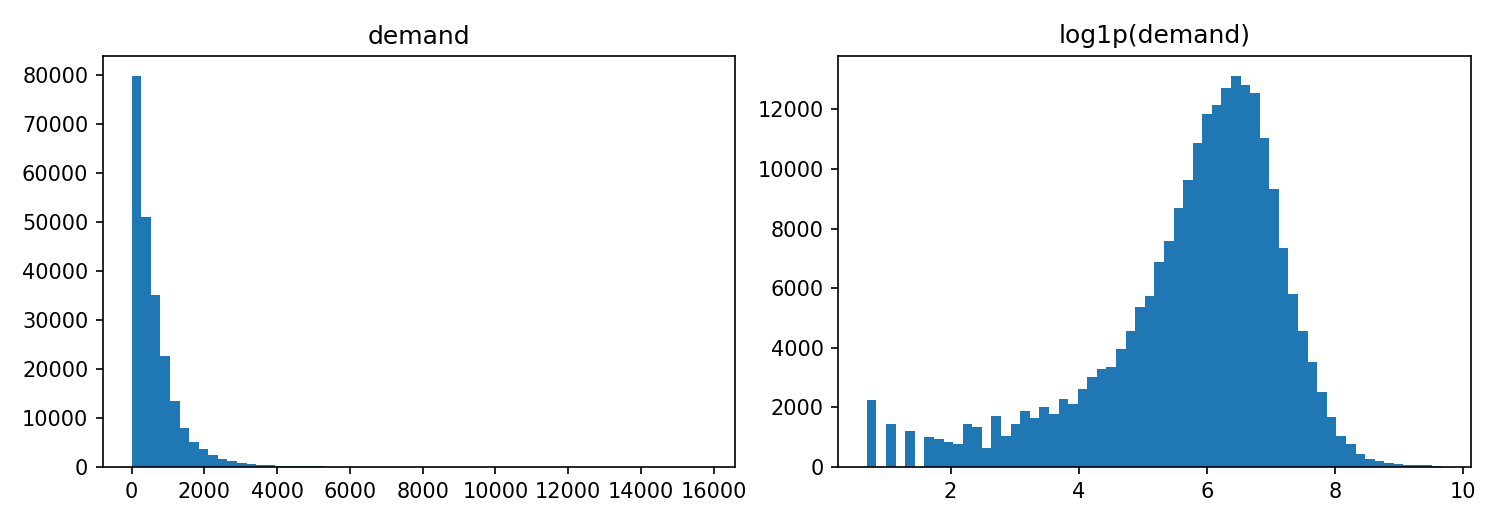
\includegraphics[width=0.85\linewidth]{figures/04_demand_dist.png}
\caption{Distribution of monthly \texttt{Part\_3} demand across all 227,344
canonical rows: raw counts (left) and $\log(1+x)$ (right). The raw signal is
heavy-tailed with skew 4.92; the log transform is near-symmetric, confirming that
per-series scaling is required before modelling.}
\label{fig:demanddist}
\end{figure}

\paragraph{F-16 — Trusts differ in scale by more than an order of magnitude.}
Aggregating demand to the trust level exposed a wide dispersion in provider size
(\Cref{fig:trustvol}). The robust spread, measured as the ratio of the 90th to the
10th percentile of total trust demand, was $66\times$; the raw extremes gave
$2690\times$ (max/min), though this figure is inflated by early-exit trusts that
reported only a handful of months before merging. Even the robust $66\times$ spread
means the largest clients carry roughly two orders of magnitude more signal than the
smallest. For cross-silo federation this is decisive: naive FedAvg weighting by
example count would let the biggest trusts steer the shared model, so \emph{size-aware
aggregation weighting} (D-03) is required to keep small clients represented. The
combination of shared structure (Stage~6) and heterogeneous scale is exactly the
regime in which personalised federated learning is expected to beat both a single
global model and isolated per-trust models.

\begin{figure}[H]
\centering
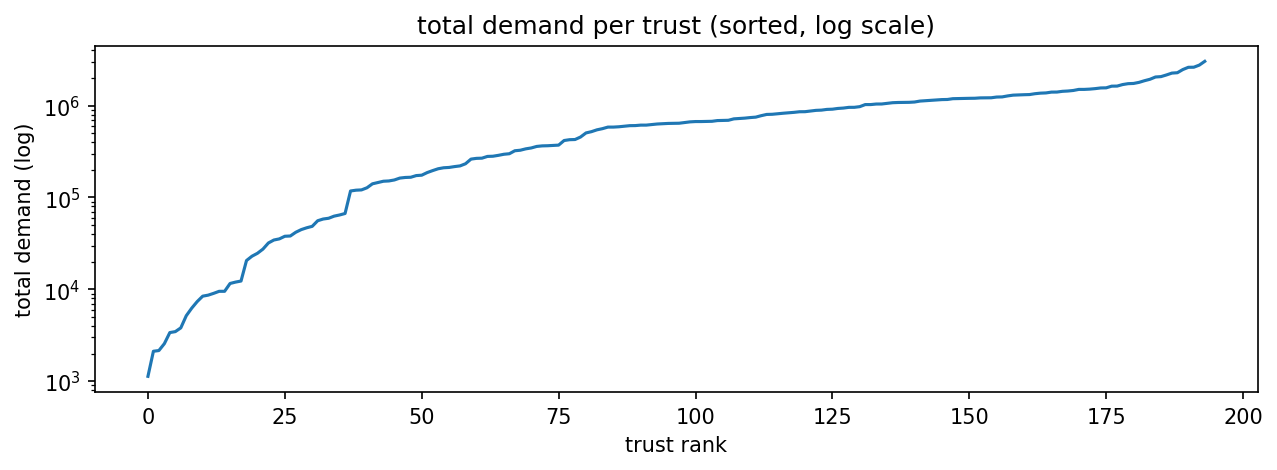
\includegraphics[width=0.85\linewidth]{figures/04_trust_volume.png}
\caption{Total \texttt{Part\_3} demand per NHS trust, sorted descending, on a
logarithmic vertical axis. The robust 90/10 percentile spread is $66\times$; the
raw max/min ratio is $2690\times$ (inflated by early-exit trusts).}
\label{fig:trustvol}
\end{figure}

\paragraph{F-17 — Demand concentrates in a handful of departments, but every
department is widely offered.} Ranking the 24 treatment functions by total demand
over the window (keyed on the stable \emph{code}, not the drifting name) gave the
leaders in \Cref{tab:topdept}. Ophthalmology (\texttt{C\_130}) led by code at
13.02\,M, followed by the catch-all ``Other'' service groupings (\texttt{X01},
\texttt{X02}, \texttt{X05}) and the surgical specialties Trauma \& Orthopaedic
(\texttt{C\_110}) and Gynaecology (\texttt{C\_502}). Coverage was broad rather than
sparse: the most common department, \texttt{X01} ``Other'', was offered by 189 of
194 trusts, the rarest, \texttt{C\_150}, by 61, and \emph{every} department appeared
in at least 61 trusts. This matters for the per-department forecaster: each shared
departmental model can draw on dozens of client silos, so no department is
data-starved at the federation level even where an individual trust does not offer
it.

\begin{table}[H]
\centering
\caption{Largest departments by total demand (by code) over 2018-04--2026-03.}
\label{tab:topdept}
\begin{tabular}{llr}
\toprule
Code & Treatment function & Total demand \\
\midrule
\texttt{C\_130} & Ophthalmology            & 13,019,148 \\
\texttt{X01}    & Other                    & 12,541,077 \\
\texttt{X02}    & Other -- Medical         & 9,759,797 \\
\texttt{X05}    & Other -- Surgical        & 7,910,330 \\
\texttt{C\_110} & Trauma \& Orthopaedic    & 7,677,829 \\
\texttt{C\_502} & Gynaecology              & 6,805,855 \\
\bottomrule
\end{tabular}
\end{table}

\paragraph{F-18 — The balanced client panel trades strictness against size.}
Requiring a trust to report in all 96 months yielded 125 fully balanced trusts;
relaxing the presence threshold recovered more clients at the cost of some gaps
(\Cref{tab:panel}). The recommended day-one client panel (D-03) is the 125 trusts
present in all 96 months, with the $\geq$90-month (139 trusts) and $\geq$84-month
(146 trusts) sets held as documented alternatives should the supervisor prefer wider
coverage over a strictly complete panel.

\begin{table}[H]
\centering
\caption{Balanced panel by presence strictness.}
\label{tab:panel}
\begin{tabular}{lr}
\toprule
Presence threshold & Trusts \\
\midrule
$\geq$96 months (complete) & 125 \\
$\geq$90 months            & 139 \\
$\geq$84 months            & 146 \\
\bottomrule
\end{tabular}
\end{table}

\paragraph{F-19 — The provider hierarchy is shallow and usable for hierarchical
aggregation.} On the latest-month (2026-03) parent mapping the 194 trusts grouped
into 42 ICBs (\Cref{tab:icb}). Trusts per ICB ranged from 1 to 13 with a median of
3, so most ICBs aggregate a small handful of clients --- a natural intermediate tier
for optional trust\,$\rightarrow$\,ICB\,$\rightarrow$\,region hierarchical
aggregation. The raw union of parent codes over the full window was 56 rather than
42; this is not genuine growth but an artefact of the July-2022 CCG$\rightarrow$ICB
parent-code changeover, which is why the hierarchy is anchored on the latest-month
mapping and on the provider side rather than the commissioner side.

\begin{table}[H]
\centering
\caption{Provider hierarchy on the 2026-03 mapping.}
\label{tab:icb}
\begin{tabular}{lr}
\toprule
Quantity & Value \\
\midrule
ICBs (latest-month mapping)   & 42 \\
Trusts per ICB, minimum       & 1 \\
Trusts per ICB, median        & 3 \\
Trusts per ICB, maximum       & 13 \\
Raw parent-code union (window) & 56 \\
\bottomrule
\end{tabular}
\end{table}

% ===== section: temporal =====
\subsection{Temporal Structure}\label{sec:temporal}

Before designing the forecaster, the temporal signature of a single trust$\times$treatment-function series was examined to confirm that RTT demand is genuinely predictable from its own past and to expose the distortion the pandemic imposes on naive time-series diagnostics.

\textbf{F-20 (strong month-to-month persistence, but an annual cycle masked by the COVID regime shift).} The busiest series in the canonical table --- provider \texttt{RP6}, department \texttt{C\_130} (Moorfields Eye Hospital, Ophthalmology) --- is one of the 1{,}412 series observed in all 96 months, so its autocorrelation function (ACF) can be estimated on a complete, gap-free record. On the raw series the lag-1 autocorrelation is $0.80$, evidencing strong short-run persistence: next month's demand is largely explained by recent months. This is the property a windowed forecaster exploits, and it justifies a modest input window of past months rather than a long-memory model. In contrast, the lag-12 autocorrelation is only $-0.01$, which would naively suggest \emph{no} annual cycle (\Cref{fig:acf}). This near-zero value is an artefact, not a fact about seasonality: the 2020 collapse and subsequent recovery (Section~\ref{sec:rel}) inject a large low-frequency regime shift into the raw series that swamps the comparatively small year-on-year seasonal term. The apparent absence of seasonality at lag 12 is therefore \emph{masked}, not real --- a point reconciled at panel scale in finding F-23 below. Practically, this means the forecaster must be given an explicit COVID regime feature and, ideally, deseasonalised or calendar-augmented inputs, so that the annual structure is recoverable rather than buried under the pandemic trend.

\begin{figure}[H]\centering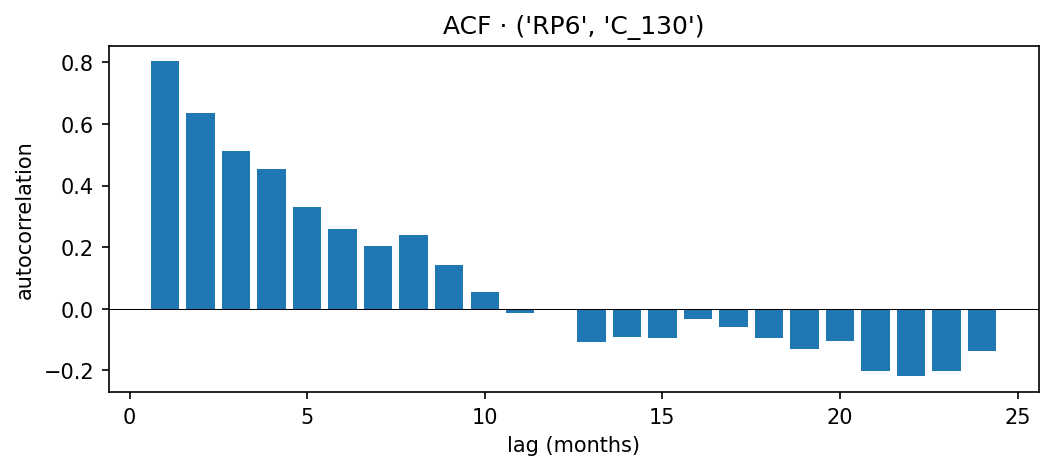
\includegraphics[width=0.85\linewidth]{figures/05_acf_busiest.png}\caption{Autocorrelation function of the busiest raw series (\texttt{RP6}$\times$\texttt{C\_130}, Moorfields Ophthalmology, complete 96/96 months). Lag-1 autocorrelation is $0.80$ (strong persistence); the lag-12 term is $-0.01$, with the annual cycle masked by the COVID regime shift rather than absent.}\label{fig:acf}\end{figure}

\textbf{Train/test split.} To support honest back-testing under this regime, a fixed chronological hold-out was fixed at the EDA stage: the first 84 months, 2018-04--2025-03, form the training window, and the final 12 months, 2025-04--2026-03, are held out for evaluation. A last-12-months hold-out keeps the split leakage-free (no future information enters training), spans a full seasonal year so that seasonal skill is actually tested, and mirrors the operational task of forecasting the year ahead. This split is reused identically across every client so that per-trust models and the federated model are compared on the same horizon.

\subsection{Cross-Series Relationships}\label{sec:rel}

Whereas Section~\ref{sec:temporal} looked within one series, the federated design question is a cross-series one: do trusts share enough structure that a jointly trained model can beat isolated per-trust models? Four findings characterise that shared structure.

\textbf{F-21 (a national collapse--recovery--growth trajectory common to all series).} Aggregating the canonical demand nationally, the new-RTT signal falls from a baseline of 1{,}544{,}011 in 2018-04 to a trough of 474{,}295 in 2020-04 --- roughly $31\%$ of baseline --- before recovering to 1{,}783{,}457 by 2026-03, about $116\%$ of the pre-pandemic level. The same collapse, rebound, and growth-above-baseline shape is visible in the busiest, median, and sparsest sample series alongside the national line (\Cref{fig:samples}). A shock of this magnitude, shared across the panel, is precisely the kind of common signal that federated aggregation can learn once and share, rather than each trust having to relearn it from its own limited history.

\begin{figure}[H]\centering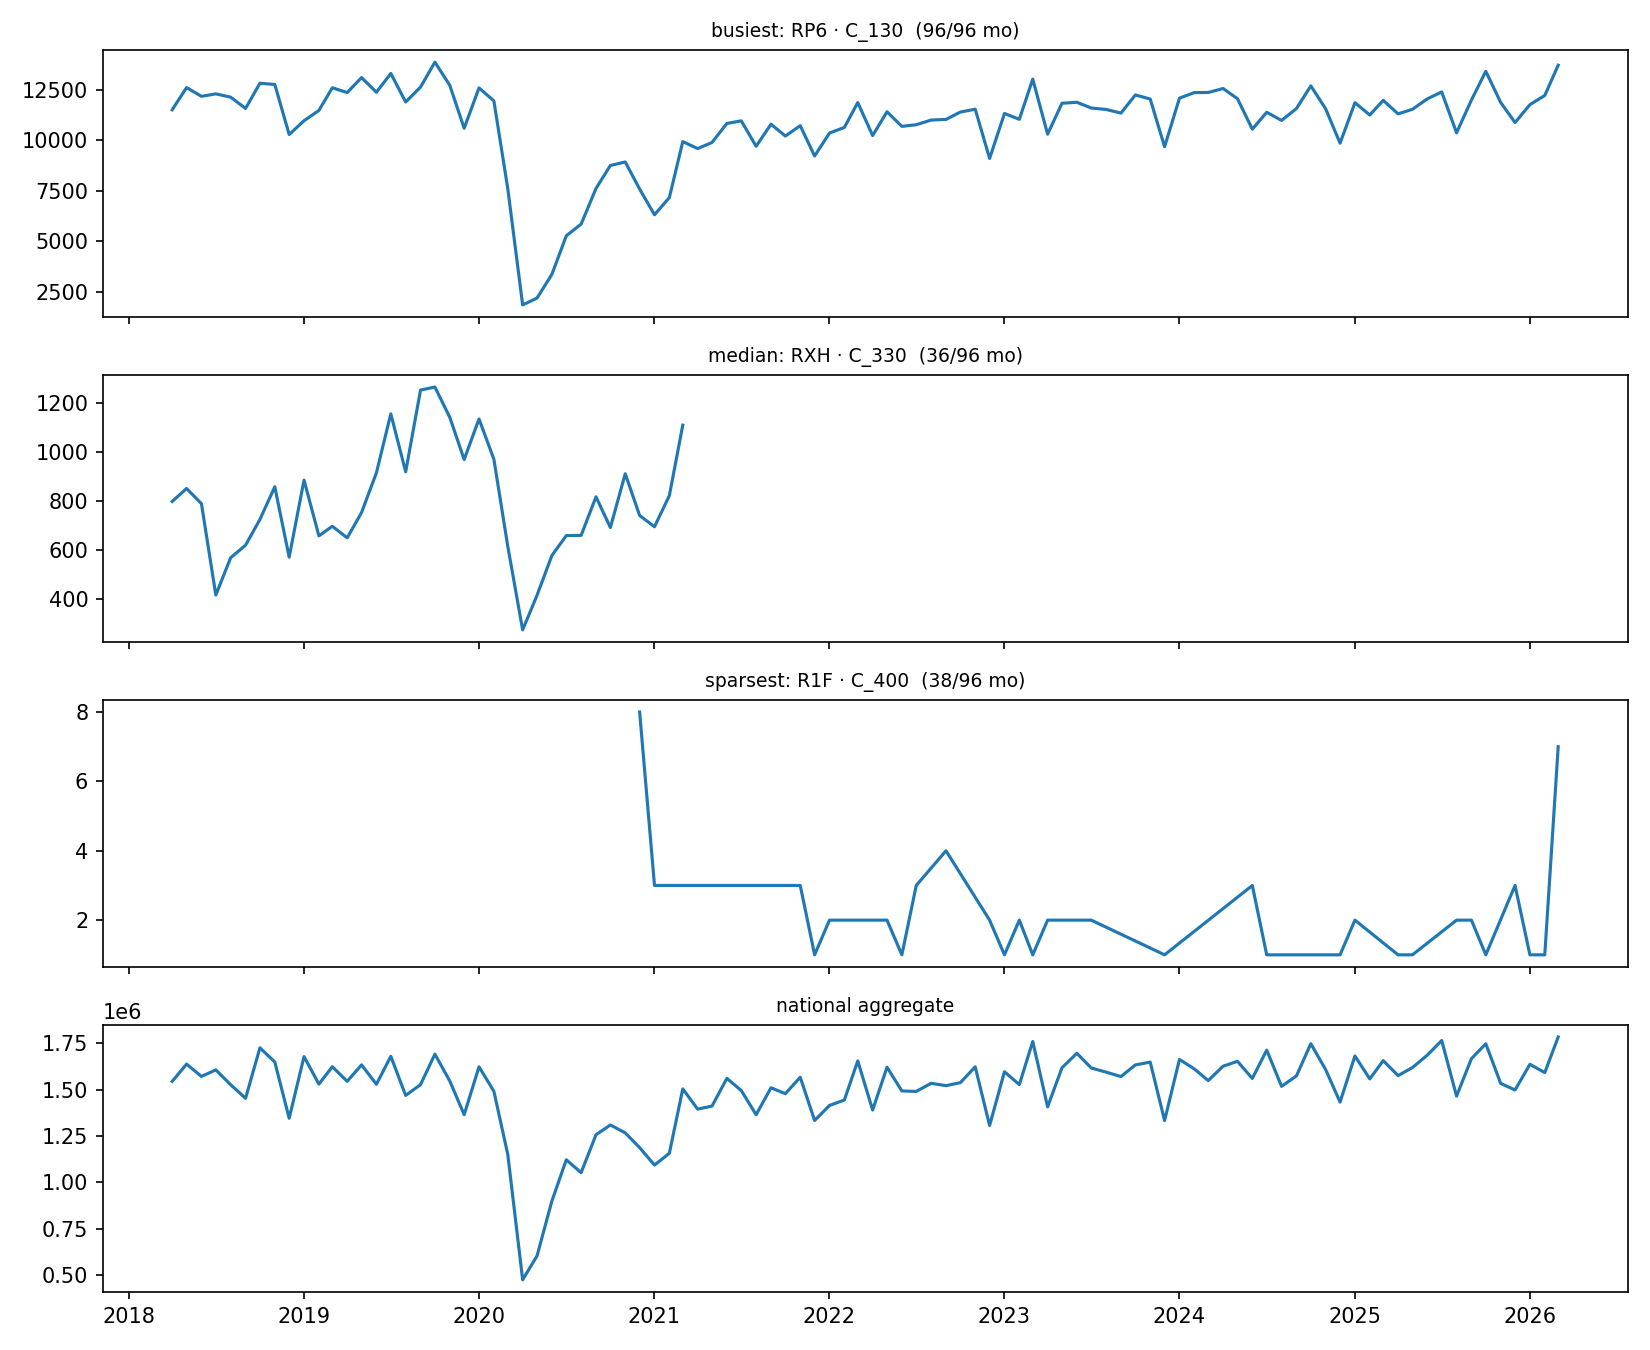
\includegraphics[width=0.85\linewidth]{figures/06_sample_series.png}\caption{Sample monthly demand series (busiest, median, and sparsest trust$\times$department series) against the national aggregate, 2018-04--2026-03. The COVID collapse to $\sim$31\% of baseline in 2020-04, recovery, and growth to $\sim$116\% of baseline are common to all.}\label{fig:samples}\end{figure}

\textbf{F-22 (a stable within-year seasonal profile).} Restricting to the post-recovery window (2022 onwards) to avoid the pandemic distortion identified in F-20, a clear calendar-month seasonality emerges: demand is lowest in December, April, and August, and highest in February, January, and March (\Cref{fig:moy}). The winter peak and the March spike --- the latter coinciding with the fiscal year-end --- are operationally meaningful and repeatable, and they motivate encoding month-of-year as a calendar feature (sine/cosine or one-hot) in the forecaster input.

\begin{figure}[H]\centering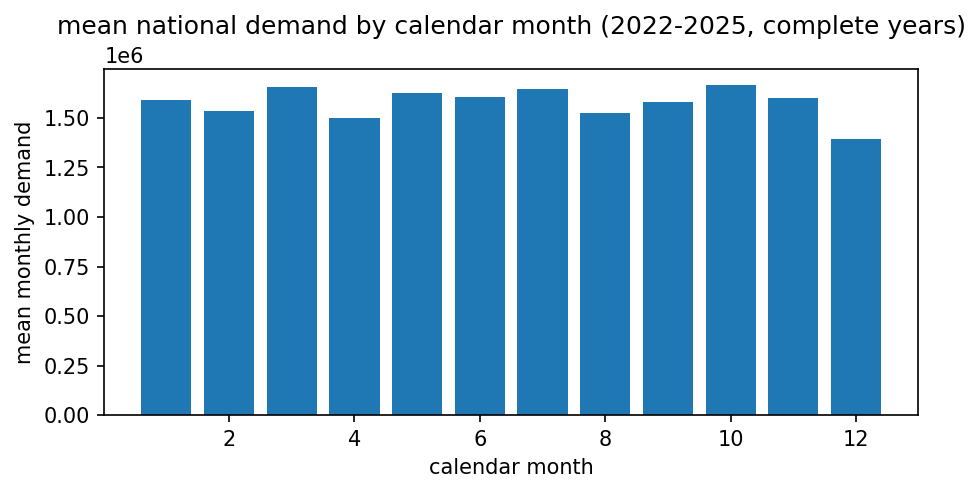
\includegraphics[width=0.85\linewidth]{figures/06_month_of_year.png}\caption{Calendar-month seasonality of new-RTT demand (2022 onwards). Lowest months are December, April, and August; highest are February, January, and March (winter peak plus March fiscal year-end).}\label{fig:moy}\end{figure}

\textbf{F-23 (the annual cycle is real at panel scale, reconciling F-20).} The near-zero lag-12 autocorrelation of the single busiest raw series (F-20) is not evidence against seasonality. Across the panel, the lag-12 autocorrelation exceeds $0.3$ in 940 of the 2{,}464 series with at least 48 months of history --- $38\%$ of eligible series. A meaningful annual cycle is therefore present in a large fraction of series; it is merely masked in individual raw series by the COVID regime shift, exactly as F-20 anticipated. This is a positive signal for federated learning: seasonality is a shared, transferable regularity that a jointly trained model can capture even for trusts whose own raw ACF is contaminated by the pandemic step.

\textbf{F-24 (synchronous cross-trust co-movement).} For the largest department, \texttt{C\_130}, the 20 largest trusts move together: the median pairwise correlation of their monthly \emph{changes} is $0.63$ (\Cref{fig:crosscorr}). Strong, synchronous co-movement indicates that trusts respond to common national shocks (funding, policy, the pandemic) rather than idiosyncratic local dynamics alone. Combined with the heterogeneous scale documented earlier (a robust $66\times$ spread across trusts) and varying departmental case-mix, this is the regime in which \emph{personalised} federated learning is expected to dominate: the shared shocks give a common structure worth aggregating (favouring FedAvg/FedProx over isolated per-trust models), while the scale and case-mix heterogeneity make a single global model insufficient (favouring per-client personalisation and size-aware weighting).

\begin{figure}[H]\centering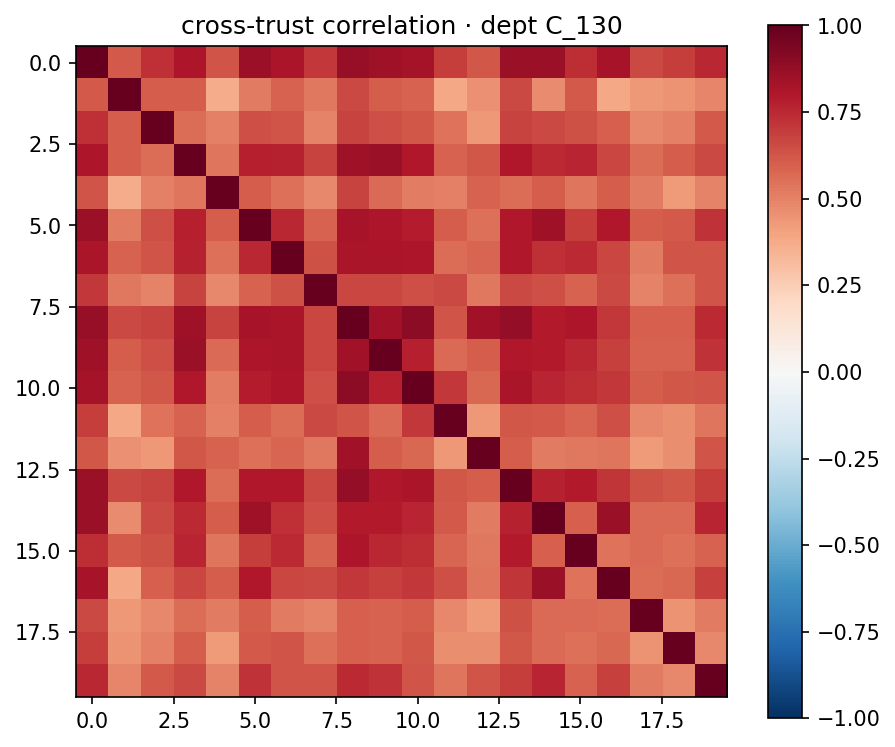
\includegraphics[width=0.85\linewidth]{figures/06_crosstrust_corr.png}\caption{Pairwise correlation of monthly demand changes across the 20 largest trusts for department \texttt{C\_130}. The median pairwise correlation is $0.63$, indicating strong shared national shocks.}\label{fig:crosscorr}\end{figure}

\textbf{Data note (key on code, not name).} Treatment-function \emph{codes} are stable across the eight-year window, but their \emph{names} drift between reporting eras: for example, \texttt{C\_130} carries at least two name spellings, and aggregating by code yields a total of about 13.0M versus only 8.3M under its latest name alone. Similarly, the \texttt{X01} ``Other'' code spans only 36 months as the X-code taxonomy shifted mid-window. Consequently the canonical department key was fixed on the \emph{code} rather than the name; keying on the name would silently fragment a single department's history and corrupt every downstream per-department series the forecaster is trained on.

% ===== section: outdisc =====
\subsection{Outliers}\label{sec:outliers}

Stage~7 screened every trust\,$\times$\,treatment-function series with at least 36 months of history for anomalous points, using a robust rolling-median plus median-absolute-deviation (MAD) z-score and a threshold of $|z|>4$. This procedure raised \textbf{4{,}183 robust flags} across the panel (F-25). The robust estimator was chosen deliberately: with a demand distribution skewed at 4.92 and a genuine COVID regime shift in the data, a classical mean/standard-deviation rule would have been dragged by the very shocks it was meant to detect, whereas the rolling median and MAD remain stable under both heavy right tails and a sustained level change.

The flags are not distributed evenly in time. The six most-flagged calendar months (\Cref{tab:outliers}, left) are dominated by the pandemic onset --- 2020-04 (354 flags) and 2020-05 (218 flags) alone account for 572 of the 4{,}183 flags --- followed by 2023-12 (209 flags), which coincides with the December~2023 industrial action, and by a cluster of winter and fiscal year-end months (2018-12, 2021-03, 2022-03). This temporal concentration confirms that the anomalies are overwhelmingly \emph{systemic} events shared across trusts rather than idiosyncratic per-series noise, which is precisely the signal a federated model must be told to treat as regime, not as data to fit.

A first-pass classification of the flags (\Cref{tab:outliers}, right) separated 1{,}961 upward spikes, 1{,}329 downward drops, and 893 COVID-regime points; unsupervised clustering of the flagged months independently recovered the COVID window as 2020-03--2021-03 (F-26), agreeing with the national-aggregate collapse and recovery seen in Stage~6. Every flag was written to an audit register at \texttt{reports/tables/07\_outlier\_register.csv}. Consistent with decision D-05, \emph{nothing was deleted}: COVID points become a binary regime-flag feature and are kept; reporting spikes, drops, and zero-blips are flagged and excluded from scaler fitting only, but are kept in the series; and genuine demand surges are left untouched. The register is therefore the complete, reversible provenance trail for every anomaly, and no observation is silently discarded before the forecaster sees it.

\begin{table}[H]
\centering
\caption{Outlier flags: the six most-flagged calendar months (left) and the first-pass class counts of the 4{,}183 robust flags (right). Flags were raised at $|z|>4$ on a rolling-median/MAD robust z-score over series with $\geq 36$ months.}
\label{tab:outliers}
\begin{tabular}{lr}
\toprule
Month & Flags \\
\midrule
2020-04 & 354 \\
2020-05 & 218 \\
2023-12 & 209 \\
2018-12 & 133 \\
2021-03 & 115 \\
2022-03 & 110 \\
\bottomrule
\end{tabular}
\qquad
\begin{tabular}{lr}
\toprule
Class & Flags \\
\midrule
Spike & 1{,}961 \\
Drop & 1{,}329 \\
COVID & 893 \\
\midrule
Total & 4{,}183 \\
\bottomrule
\end{tabular}
\end{table}

\section{Discussion}\label{sec:discussion}

The central question this analysis was designed to answer is not merely whether NHS RTT demand can be forecast, but whether its structure justifies a \emph{personalised federated} approach in preference to the two simpler baselines: a single global model trained as if all trusts were interchangeable, and a fleet of isolated per-trust models each ignoring its peers. The evidence assembled across Stages~2--7 points consistently to the middle option, because the data exhibits strong shared structure \emph{and} strong client-specific heterogeneity at the same time.

\paragraph{Shared national structure --- the case for pooling.} Three independent measurements show that trusts do not move independently. First, the pandemic shock was synchronous: the national Part\_3 aggregate fell from a 2018-04 baseline of 1,544,011 new periods to a 2020-04 trough of 474,295 (about 31\% of baseline), and this collapse-then-recovery is visible in every sample series rather than in a few outliers, recovering to 1,783,457 (about 116\% of baseline) by 2026-03. Second, co-movement persists outside the shock: across the twenty largest trusts in the busiest department (Ophthalmology, \texttt{C\_130}), the median pairwise correlation of monthly demand \emph{changes} is 0.63, indicating a large common component in month-to-month dynamics. Third, seasonality is a shared calendar effect: 940 of 2{,}464 series with $\geq 48$ months of history (38\%) carry a lag-12 autocorrelation above 0.3, with demand systematically lowest in December, April and August and highest in February, January and March (winter pressure plus the March fiscal year-end). This common structure --- national shocks, correlated dynamics, and a shared annual cycle --- is exactly what a federated model can learn once, from the pooled experience of many trusts, far more reliably than any single site could estimate from its own short history.

\paragraph{Client heterogeneity --- the case against a single global model.} The same data is strongly non-homogeneous across clients. The robust cross-trust scale spread is $66\times$ (the 90th-to-10th-percentile ratio of trust demand), and the raw demand distribution is heavily right-skewed (skew 4.92, median 428 against a maximum of 15{,}807), so any model that shares parameters across trusts on the raw scale would be dominated by a handful of very large sites. Casemix also differs: the number of departments a trust offers ranges from 1 to a maximum of 24 (median 20), the most common department (\texttt{X01}) is offered by 189 of 194 trusts while the rarest (\texttt{C\_150}) is offered by only 61, and roughly 1{,}400 trust\,$\times$\,department pairs never appear at all. A single global forecaster cannot reconcile a small district trust running one specialty with a national tertiary centre running the full slate. These differences make \emph{per-series standardisation} and \emph{size-aware federated weighting} mandatory (decisions D-03/D-04), and they are the concrete reason personalisation layers on top of FedAvg/FedProx are expected to outperform a purely global fit.

Taken together, the coexistence of a large shared component (correlation 0.63, synchronous COVID collapse, 38\% seasonal) with large client-specific differences ($66\times$ scale, divergent casemix) is the textbook regime in which personalised cross-silo federated learning should beat both a single global model and isolated local models, while never moving a trust's raw records off-site.

\paragraph{Non-stationarity from trust mergers.} The client population itself is not fixed. Across the four sentinel months the count of NHS trusts \emph{shrinks} from 184 to 149 even as the total provider count \emph{grows} from 417 to 533, and in the full window 45 trusts exit early against only 11 that enter late --- a pattern dominated by mergers and consolidation rather than genuine service closure. This organisational non-stationarity is why the client roster was fixed by a balanced-panel choice (125 of 194 trusts reporting in all 96 months, with 139 and 146 available at the relaxed $\geq 90$- and $\geq 84$-month thresholds) rather than by imputing the histories of trusts that ceased to exist under their old code. For the federation this means the participant set must be treated as a design decision with an explicit stability criterion, not as a property that can be assumed constant.

\paragraph{Structural-zero sparsity.} Sparsity in this data is structural, not missingness to be repaired. Of 3{,}243 trust\,$\times$\,department series, 1{,}412 (44\%) are complete over all 96 months while 1{,}831 are gappy (median 60 of 96 months present), and the roughly 1{,}400 pairs that never appear reflect services a trust simply does not provide. The canonical table contains 0 NaN and 0 literal-zero demand rows; absence is encoded as the row not existing, and NaN arises only when a series is reindexed to full monthly frequency. Accordingly (decision D-02) reporting gaps are kept as NaN and skipped by the forecaster's input window, structural zeros are never imputed, and no NaN is ever filled with 0 --- preventing a client from learning a spurious ``zero demand'' signal for a specialty it never ran.

\paragraph{The ICB hierarchy as an aggregation backbone.} Finally, the provider-parent field supplies a ready-made intermediate tier: 42 Integrated Care Boards on the latest-month mapping, with a median of 3 trusts per ICB (minimum 1, maximum 13, largest QYG with 13). This hierarchy is what makes trust\,$\rightarrow$\,ICB\,$\rightarrow$\,region aggregation feasible, allowing the coordinator to pool updates from small or sparse trusts within their ICB to stabilise their forecasts before contributing to the national model --- a natural remedy for the sparsity and scale problems above. The region tier is not present in the RTT files and must be attached from an external provider\,$\rightarrow$\,region lookup, and the parent-code union of 56 over the window (versus 42 latest) is an artefact of the July~2022 CCG\,$\rightarrow$\,ICB changeover, confirming the decision to anchor the hierarchy on the provider side. Downstream of the forecaster, the agentic plane will branch on provider type --- allocating capacity to directable NHS trusts and commissioning (buying) activity from independents --- but that branching sits outside the forecasting task characterised here, which treats every trust uniformly as a federated client.

% ===== section: recoapp =====
\section{Recommendations and Decisions}\label{sec:reco}

The exploratory analysis produced five locked decisions, D-01 through D-05, each traceable to a specific finding in the register of \Cref{sec:findings}. \Cref{tab:decisions} records them; every rule was either executed against all 96 monthly files or fixed as a modelling-time specification.

\begin{table}[H]
\centering
\caption{Locked decisions carried out of the EDA. D-01 was executed to the canonical parquet; D-04 and D-05 are model-time specifications.}
\label{tab:decisions}
\small
\begin{tabular}{@{}l p{0.82\linewidth}@{}}
\toprule
ID & Locked decision \\
\midrule
D-01 & \textbf{Loader spec.} Read only the 9 canonical columns; parse \texttt{Period} case-insensitively; set \texttt{demand} = \texttt{Total All} where \texttt{RTT Part Type} $=$ \texttt{Part\_3}; keep NHS trusts (\texttt{R\#\#}); drop \texttt{C\_999}; sum over the commissioner split; coerce \texttt{demand} to numeric. Executed $\rightarrow$ 227,344 rows. \\
D-02 & \textbf{Missingness rules.} Entry/exit is handled by the panel choice, not imputation; reporting gaps are kept as NaN (the forecaster window skips them); structural zeros are never imputed; literal zeros are kept; NaN is never filled with 0. \\
D-03 & \textbf{Client panel.} Use the 125 trusts present in all 96 months (alternatives: 139 at $\geq 90$ months, 146 at $\geq 84$ months); restrict to departments offered by a high share of panel trusts; per-series scaling and size-aware federated weighting are mandatory. \\
D-04 & \textbf{Transforms.} Per-series standardisation fitted on TRAIN only; input window of 12--24 months plus calendar features (month sin/cos or one-hot); hold out the last 12 months; add a COVID regime flag for 2020-03--2021-03; no leakage. \\
D-05 & \textbf{Outlier actions.} COVID points $\rightarrow$ regime-flag feature, KEEP; reporting spike/drop/zero-blip $\rightarrow$ flag and exclude from scaler fitting, KEEP; genuine surge $\rightarrow$ keep untouched; nothing deleted; the register is the audit trail. \\
\bottomrule
\end{tabular}
\end{table}

\paragraph{Recommended path.} The analysis supports a concrete, defensible configuration for the first federated experiments. The federation client set should be the \textbf{125-trust balanced panel} (trusts reporting in all 96 months, 2018-04--2026-03), which removes the confounding of late entry (11 trusts) and early exit (45 trusts, dominated by merger-driven consolidation) without any imputation. Because trust demand spans a factor of $66\times$ at the robust $p90/p10$ level and the pooled demand distribution is heavily right-skewed (skew 4.92, median 428 versus max 15{,}807), \textbf{per-series standardisation} (fitted on TRAIN only) together with \textbf{size-aware client weighting} is required so that a few very large trusts do not dominate the shared model. The forecaster should consume an \textbf{input window of 12--24 months} plus calendar features, and be evaluated on a \textbf{last-12-months back-test} (train 2018-04--2025-03, test 2025-04--2026-03), which holds out a full seasonal cycle. Hierarchical aggregation should be anchored on the \textbf{42-ICB latest-month (2026-03) mapping} rather than the raw 56-code union, since the larger figure is an artefact of the July-2022 CCG$\rightarrow$ICB parent-code changeover rather than a real growth in commissioner parents.

The joint evidence justifies the federated framing. Trusts move together under shared national shocks --- the synchronous 2020-04 collapse and a median pairwise monthly-change correlation of 0.63 across the twenty largest Ophthalmology providers --- giving common structure a global model can exploit; yet they differ sharply in scale ($66\times$) and case-mix (departments offered per trust range 1--24). This combination of shared signal and per-client heterogeneity is precisely the regime in which \textbf{personalised} federated learning (FedAvg / FedProx with personalisation, optionally trust$\rightarrow$ICB$\rightarrow$region hierarchical aggregation) is expected to beat both a single pooled model and isolated per-trust models.

\subsection{Open Questions for the Supervisor}
Four choices are analyst-bounded but ultimately require supervisor judgement, because they trade client count against panel cleanliness:
\begin{enumerate}[nosep]
  \item \textbf{Panel strictness.} Adopt the strict $\geq 96$-month panel (125 trusts), or relax to $\geq 90$ months (139 trusts) or $\geq 84$ months (146 trusts) to buy roughly 11--21 additional clients at the cost of some ragged history.
  \item \textbf{COVID span.} Confirm the regime window as 2020-03--2021-03 (supported by the outlier clustering and the 940-of-2464 lag-12 signal), or widen/narrow it; this defines both the regime-flag feature and which points are excluded from scaler fitting.
  \item \textbf{Small-trust inclusion.} Decide whether the smallest, early-exit trusts (which inflate the raw $\max/\min$ spread to $2690\times$) are kept as clients or excluded, given size-aware weighting will already down-weight them.
  \item \textbf{Department coverage threshold.} Fix the minimum share of panel trusts that must offer a department for it to enter the federated model (every department is offered by at least 61 of 194 trusts; the most common, X01, by 189).
\end{enumerate}

\section{Conclusion}\label{sec:conclusion}
The EDA gate is open. All 96 monthly RTT files (2018-04--2026-03) were verified for schema and integrity, reduced through a fully ledgered filter (raw 17{,}355{,}150 rows $\rightarrow$ 227{,}344 canonical rows), and characterised for coverage, scale, seasonality, sparsity, hierarchy and outliers. National Part\_3 trust totals were externally validated on four sentinel months (computed $=$ expected, 4/4), the entire analysis reruns restart-and-run-all clean (57 cells, 0 errors), and the five decisions D-01--D-05 are logged with their supporting findings. The data is now understood well enough to (i) fix the client panel and (ii) design the forecaster. The immediate next steps are to build the swappable forecaster interface behind \texttt{get\_params}/\texttt{set\_params} and to stand up the Flower cross-silo federated loop over the recommended 125-trust panel, keeping every trust's raw data on-site as required.

\appendix
\section{Findings Register}\label{sec:findings}
\Cref{tab:findings} consolidates the 26 EDA findings (F-01--F-26) across the schema, canonical-build, missingness, characteristics, transform, relationship and outlier stages. Each is a verified statement drawn directly from the analysis notebook.

\begin{table}[H]
\centering
\caption{EDA findings register, F-01 through F-26.}
\label{tab:findings}
\small
\begin{tabular}{@{}l p{0.86\linewidth}@{}}
\toprule
ID & Finding \\
\midrule
F-01 & Column layout steps 69$\rightarrow$121 exactly at 2021-04 (36 months at 69 cols, 60 at 121); the extra 52 columns extend the weekly wait-band histogram from 52 to 104 weeks. \\
F-02 & RTT part types \{Part\_1A, Part\_1B, Part\_2, Part\_2A, Part\_3\} are identical across all eras; \texttt{Part\_3} is the exact demand label and Part\_2A is present from 2018-04. \\
F-03 & Treatment functions grow from 20 to 24 across the window; the \texttt{C\_999} aggregate "Total" specialty is present in every era and is dropped. \\
F-04 & NHS trusts (\texttt{R\#\#}) per sentinel are 184 / 173 / 170 / 149 of 417 / 414 / 431 / 533 providers; trust count shrinks (mergers) while providers grow; code lengths are strictly \{3,5\}. \\
F-05 & \texttt{Period} month case is non-monotonic (April / APRIL / APRIL / March); case-insensitive parsing recovers the month and the title-cased month matches the filename 4/4. \\
F-06 & \texttt{Total All} is dtype int64 in every era with 0 NaN. \\
F-07 & External validation of national Part\_3 trust totals: computed $=$ expected 4/4 (2018-04 $=$ 1{,}544{,}011; 2020-04 $=$ 474{,}295; 2021-04 $=$ 1{,}394{,}578; 2026-03 $=$ 1{,}783{,}457). \\
F-08 & Full-window audit: the 7 canonical columns present 96/96, a single parent-header variant, and \texttt{Part\_3} with numeric \texttt{Total All} present 96/96 --- 0 problem files. \\
F-09 & Filter ledger (96 months): raw 17{,}355{,}150 $\rightarrow$ Part\_3 3{,}614{,}127 (20.8\%) $\rightarrow$ trusts 2{,}987{,}812 (82.7\% of Part\_3) $\rightarrow$ drop C\_999 2{,}376{,}866 $\rightarrow$ sum commissioners $\rightarrow$ 227{,}344 rows; 0 duplicates removed. \\
F-10 & Finished table: 227{,}344 rows, 96 months, 194 trusts (union), 24 departments, 56 ICBs (raw parent-code union); saved as a 0.6 MB parquet; national totals re-validated 4/4. \\
F-11 & Balanced panel: 125 of 194 trusts report in all 96 months. \\
F-12 & 11 trusts enter late and 45 exit early; exits dominate, consistent with NHS trust mergers/consolidation. \\
F-13 & 3{,}243 trust$\times$dept series: 1{,}412 complete all 96 months (44\%) and 1{,}831 gappy (median 60/96 months). \\
F-14 & Departments offered per trust: min 1, median 20, max 24; roughly 1{,}400 trust$\times$dept pairs never appear as structural zeros. The canonical table has 0 NaN and 0 literal-zero demand rows (every row $\geq 1$); NaN arises only when a series is reindexed to full monthly frequency (\texttt{asfreq MS}). \\
F-15 & Demand distribution: mean 632.9, std 778.4, min 1, median 428, max 15{,}807, skew 4.92 (heavy right skew) --- per-series scaling is mandatory. \\
F-16 & Trust scale spread: robust $p90/p10 = 66.1\times$; $\max/\min = 2690\times$ (inflated by early-exit trusts) --- size-aware federated weighting required. \\
F-17 & Top departments by total demand: \texttt{C\_130} Ophthalmology 13.0M by code; \texttt{X01} ``Other'' 12.5M; \texttt{X02} 9.76M; \texttt{X05} 7.91M; \texttt{C\_110} 7.68M; \texttt{C\_502} 6.81M. Coverage: \texttt{X01} offered by 189/194 trusts, rarest \texttt{C\_150} by 61 ($\geq 61$ for all). \\
F-18 & Balanced panel by strictness: $\geq 96$ months $=$ 125 trusts, $\geq 90$ $=$ 139, $\geq 84$ $=$ 146. \\
F-19 & Hierarchy: 42 ICBs on the latest-month (2026-03) mapping (raw union 56 inflated by the July-2022 CCG$\rightarrow$ICB changeover); trusts per ICB min 1, median 3, max 13 (QYG 13, QHM 9, QOP 7). \\
F-20 & Busiest series \texttt{RP6}$\times$\texttt{C\_130} (Moorfields, Ophthalmology), complete 96/96; raw ACF lag-1 $=$ 0.80, lag-12 $=$ $-0.01$ (annual cycle masked by the COVID regime shift). Split: train 84 months / test last 12. \\
F-21 & National aggregate: baseline 2018-04 $=$ 1{,}544{,}011, trough 2020-04 $=$ 474{,}295 (31\%), latest 2026-03 $=$ 1{,}783{,}457 ($\sim$116\% of baseline) --- collapse, recovery and growth above baseline. \\
F-22 & Seasonality (2022+): lowest calendar months Dec/Apr/Aug, highest Feb/Jan/Mar (winter plus March fiscal year-end). \\
F-23 & Panel-wide annual cycle: lag-12 autocorr $> 0.3$ in 940 of 2{,}464 series (38\%) with $\geq 48$ months, reconciling the masked single-series ACF of F-20. \\
F-24 & Cross-trust co-movement (\texttt{C\_130}, 20 largest trusts, monthly changes): median pairwise correlation 0.63. Function codes are stable but names drift (\texttt{C\_130} $\geq 2$ spellings) so departments are keyed on code, not name; \texttt{X01} ``Other'' spans only 36 months. \\
F-25 & 4{,}183 robust outlier flags (rolling-median + MAD z-score, $|z| > 4$, series $\geq 36$ months); top months 2020-04 (354), 2020-05 (218), 2023-12 (209, strikes), 2018-12 (133), 2021-03 (115), 2022-03 (110). \\
F-26 & First-pass outlier classes: spike 1{,}961, drop 1{,}329, covid 893; the COVID regime window 2020-03--2021-03 is confirmed by the clustering; register at \texttt{reports/tables/07\_outlier\_register.csv}. \\
\bottomrule
\end{tabular}
\end{table}

\end{document}
